\subsection{Data Plane Strategies}

\begin{task}
\label{task:system:dataplane}
We will design and implement efficient data-plane implementations to
guarantee \blue{reachability and consistency properties}, in presence
of reconfiguration and link dynamics.
\end{task}

In translating the solution provided by the optimization engine into a
consistent and efficient data plane forwarding strategy, We build upon
recent advances in software-defined networking (SDN).  While SDN is an
``enabler,'' as it provides cleaner management abstractions and open
interfaces (e.g., via APIs such as OpenFlow~\cite{}), \ArchName
introduces unique consistency and efficiency challenges.  In
particular, in face of a dynamically changing network due to
reconfigurations, we need to ensure that (a) packets do not use
deactivated links \blue{(i.e., black holes~\cite{} are avoided)}, (b)
the network remains connected at all times, and (c) the packet latency
remains bounded. Finally, we also need a data plane strategy to: (d)
handle transient misalignment of FSO links. We note that the recent
related works either assume a {\em static}
network~\cite{cons-update,incconsupdate} or focus on a single
reconfiguration~\cite{cu-1}, and hence, are not directly applicable to
our context.

\para{\underline{(a) and (b).} Guaranteeing Correctness and Connectivity.}
Packets are routed in the network on the basis of forwarding tables,
which essentially specify, at each node, the next hop/link to use for
each destination. In a dynamic network, forwarding tables will also be
changing constantly.  Note that activation/deactivation of a link
takes a finite amount of time, and that we cannot update the tables
across all the network switches atomically (i.e., {\em at once}).
%
In face of the above challenges, we need to ensure that through every
possible intermediate state of the links and switches' tables, only
active links appear in the forwarding tables. We can ensure this by a
careful ordering of steps as suggested in our preliminary
work~\cite{hotnets}; in particular, (i) we reflect removal of links in
the forwarding tables, before actually deactivating the links, and
(ii) reflect addition of links in the tables only after the link
activation is complete. Note that the above solution ensures the
desired property even in face of multiple concurrent reconfigurations,
and irrespective of the order in which forwarding tables are updated
across the network.

In addition to above, we also need to ensure that the network remains
connected at all times. There are two possible options: (i) We
maintain a static ``backbone'' subnetwork that ensures connectivity,
or (ii) reject reconfigurations that disconnect the network. The first
approach reduces the degree of flexibility in network design and
\blue{may result in high packet latency, depending on the backbone.}
The second approach becomes challenging to implement if there are
multiple {\em concurrent} reconfigurations. There are three options to
handle concurrent reconfigurations: (i) one at a time, (ii) in batches
(i.e., queue and combine them into a single reconfiguration); and
(iii) execute each reconfiguration individually but {\em
  concurrently}. The first two options can be inefficient as large
flows have to wait until the desired link(s) become available, while
the third option requires a careful implementation to ensure
consistency. In particular, for the third option, we need to keep a
single consistent view of the network topology graph and allow only
{\em atomic} access to it (when one needs to check if deactivation of
a set of links disconnents the network). \green{Again, the above
  solutions work irrespecitve of the order in which the forwarding
  tables are updated across the network.} In our research, we will
study the performance of the above described approaches.

\begin{wrapfigure}{r}{0.3\textwidth}
\vspace{-0.4cm}
\centering
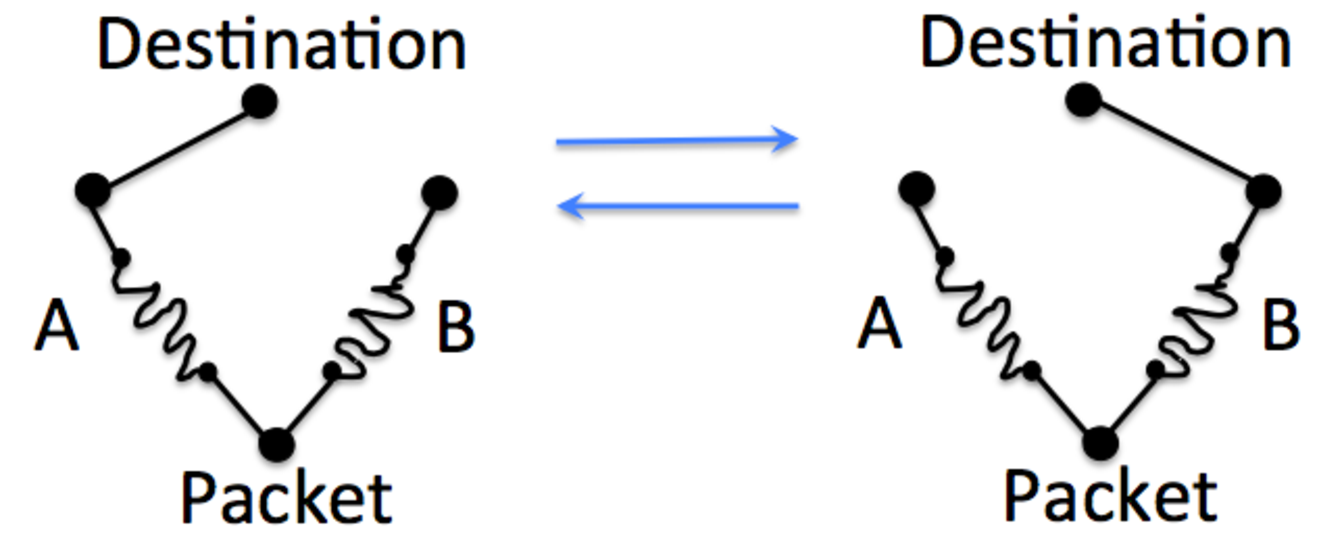
\includegraphics[width=150pt]{PPTFigs/impossible.pdf}
\caption{If the network goes back and forth between the above
  topologies (due to corresponding reconfigurations), then the packet
  will continue to ``swing'' between areas A and B -- leading to a
  forwarding ``loop''.}
\label{fig:impossible}
\end{wrapfigure}
\para{\underline{(c)} Guaranteeing Bounded Packet Latency.}  The above
strategies still do not guarantee a bounded packet latency. In fact,
in general, its {\em impossible} to avoid guarantee bounded packet
latency in general. See Figure~\ref{fig:impossible}. There are two approaches to
bound the latency of (in-flight) packets: (i) create and use a
backbone {\em static} subnetwork with bounded diameter, (ii) reject
reconfigurations to avoid high packet latency. The first approach will
require careful decision-making of {\em when} to resort to routing a
packet to the backbone (due ot its limited bisection bandwidth), while
the second approach will require an efficient and fast computation of
the impact on latency of the packets (especially, the in-flight
packets). In addition, we should formally characterize and avoid 
scenarios like the one described in Figure~\ref{fig:impossible}.

\para{\underline{(d)} Handling Misalignment of Links.} In \ArchName, even during
a static topology state, links may be temporarily unavailable because
of possible misalignment of the FSO links. \blue{Such misalignments
  are fixed in real-time by ``micro alignment'' of FSO devices, as
  suggested in Section~\ref{sec:fso}}, and the timescales of such
  micro-alignment is likely to be much smaller than the time needed to
  update rules~\cite{ddcnsdi13} through an SDN controller. In fact, it
  may even be counterproductive to report such transient link failures
  to the controller, as it may cause needless \blue{reconfigurations
    and/or update of forwarding tables}. Thus, we need appropriate
  \blue{network layer} techniques to recover from such transient link
  failures. \blue{Future SDN roadmaps have provisions for local
    recovery mechanisms analogous to similar schemes in the MPLS and
    SONET literature~\cite{}. We will explore the available
    alternatives in our research. In the absence of such features,} we
  will investigate design of a local ``lightweight'' SDN controller on
  every rack that can quickly react to such misalignments while
  relying on the global controller for longer-timescale
  reconfigurations~\cite{ddc}.
